
\documentclass[tikz, convert={outfile=\jobname.png}]{standalone}

%% In /etc/ImageMagick-6/policy.xml
% change line:
% policy domain="coder" rights="none" pattern="PDF" 
% to:
% policy domain="coder" rights="read|write" pattern="PDF"

\begin{document}

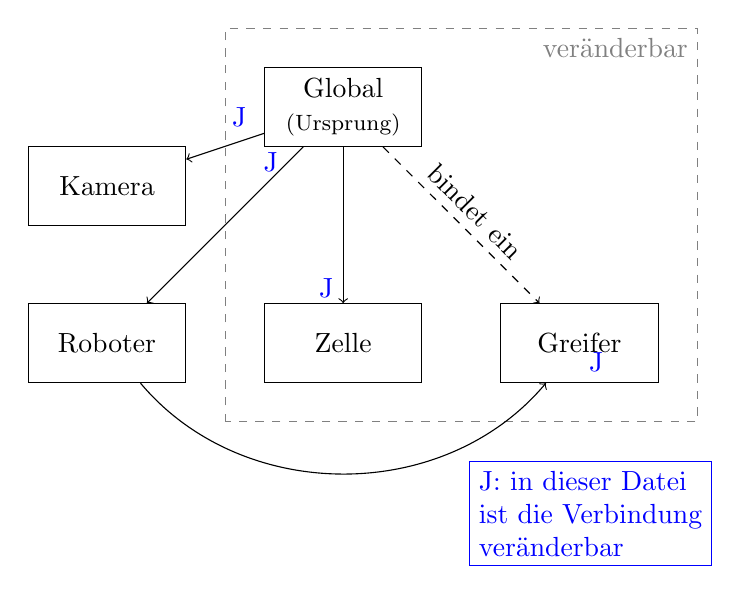
\begin{tikzpicture}[
block/.style={draw, align=center, minimum height=1cm, minimum width=2cm}]


\draw[dashed, gray] (-1.5, -1) rectangle (4.5, 4) node[below left]{ver\"anderbar};


\path (0,0) node[block](cell){Zelle};
\path (0,3) node[block](global){Global \\ \footnotesize (Ursprung)};
\path (3,0) node[block](gripper){Greifer};
\path (-3,0) node[block](robot){Roboter};
\path (-3,2) node[block](cam){Kamera};




\draw[->] (global) --(cell)node[pos=.9, left, blue]{J};
\draw[->, dashed] (global) --(gripper) node[sloped, midway, above]{bindet ein};
\draw[->] (global) --(robot)node[pos=.1, left, blue]{J};

\draw[->] (global) --(cam)node[pos=.1, above left, blue]{J};

\draw[->] (robot) to [out=-50, in=-130] (gripper)node[below right, blue]{J};


\path (1.6,-1.5)node[below right, align=left, draw, blue]{J: in dieser Datei \\ ist die Verbindung \\ ver\"anderbar};


\end{tikzpicture}


\end{document}